\section{Results}
This section analyzes the measurements collected across three experiments and three cluster sizes (3, 6 and 9 nodes), where each experiment was repeated three times with a one hour duration. For configuration and parameter details that were used to achieve these measurements, see Section~III.

\subsection{Throughput}
Table~\ref{tab:throughput} summarizes the throughput results from the linear-capacity experiment. Each node was loaded with 160 publishers using asynchronous confirms, resulting in 480, 960 and 1{,}440 total publishers for the 3, 6 and 9-node clusters respectively.

\begin{table}[h]
\centering
\caption{Summary of throughput results from the linear-capacity experiment.}
\label{tab:throughput}
\begin{tabular}{l r r r}
\hline
\textbf{Cluster} & \textbf{Mean (msgs/s)} & \textbf{Scaling Factor} & \textbf{Std Dev} \\
\hline
3 Nodes  & 98{,}134  & 1.00$\times$ & 508  \\
6 Nodes  & 210{,}785 & 2.15$\times$ & 3{,}433 \\
9 Nodes  & 304{,}867 & 3.11$\times$ & 2{,}646 \\
\hline
\end{tabular}
\end{table}

The cluster achieves approximately linear throughput scaling. Tripling the node count from 3 to 9 yields a 3.11$\times$ improvement, which is consistent with the 3$\times$ increase in cluster nodes. Since the quorum size is fixed at 3, adding nodes introduces new queues and publishers without increasing per-message replication overhead. Only three replicas must acknowledge each write regardless of cluster size, so the additional nodes contribute more publishing capacity without adding consensus overhead.

Per-node throughput remains consistent across all cluster configurations, ranging from approximately 32{,}700 msgs/s per node (3-node) to 35{,}100 msgs/s per node (6-node) and 33{,}900 msgs/s per node (9-node). Since the number of queues and publishers scales proportionally with the node count, each node handles the same workload regardless of cluster size. As a result, we see a relatively consistent per-node throughput with a low inter-run standard deviation of 508--3{,}433 msgs/s. As seen in Figure~\ref{fig:throughput_ts}, the throughput is stable across the one-hour benchmark duration.

\begin{figure}[h]
\centering
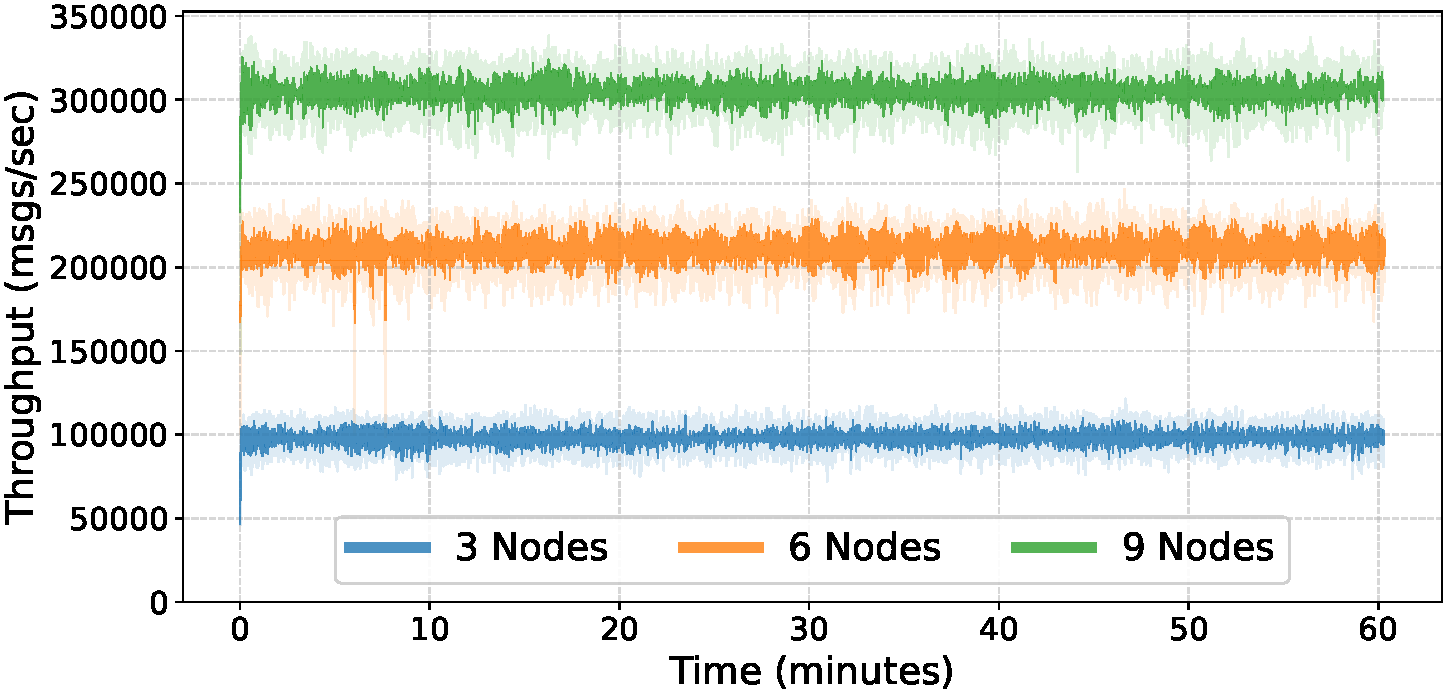
\includegraphics[width=\columnwidth]{../results/plots/6_throughput_timeseries.pdf}
\caption{Per-second throughput averaged across all three runs for each cluster size, with shaded bands showing inter-run standard deviation.}
\label{fig:throughput_ts}
\end{figure}

Figure~\ref{fig:throughput} shows the expected throughput if performance scaled linearly from the 3-node result. The error bars represent inter-run standard deviation across all our three benchmark runs. The measured values are close to the expected line, with the 6-node and 9-node clusters slightly exceeding it.

\begin{figure}[h]
\centering
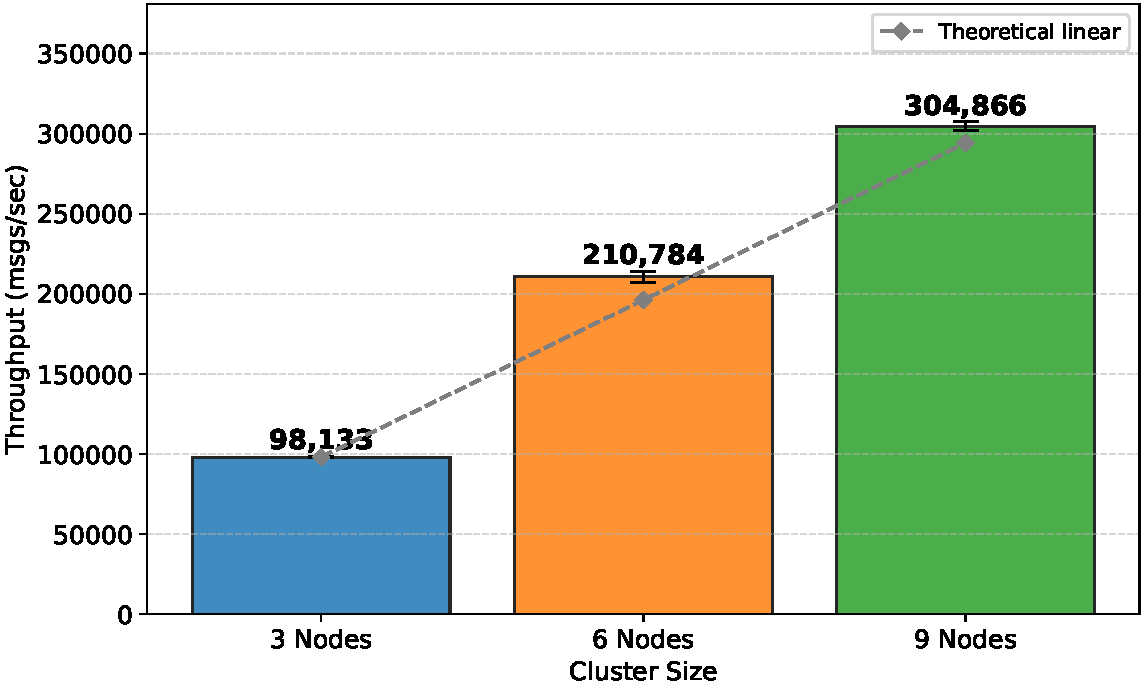
\includegraphics[width=\columnwidth]{../results/plots/1_throughput_scalability.pdf}
\caption{Mean throughput per cluster size with inter-run standard deviation error bars.}
\label{fig:throughput}
\end{figure}

\subsection{Latency Under Ideal Conditions}
\label{subsec:ideal_latency_results}
The ideal-latency experiment isolates the Raft consensus latency by using a single publisher and consumer connected directly to the queue leader node. Table~\ref{tab:ideal_latency} summarizes the results. Unlike the throughput experiment, the quorum size equals the cluster size here, so every node participates in consensus.

\begin{table}[h]
\centering
\caption{Summary of results from the ideal-latency experiment.}
\label{tab:ideal_latency}
\begin{tabular}{l c r}
\hline
\textbf{Cluster} & \textbf{Mean ($\mu$s)} & \textbf{P99 ($\mu$s)} \\
\hline
3 Nodes & 3{,}420 & 4{,}550 \\
6 Nodes & 4{,}000 & 4{,}690 \\
9 Nodes & 4{,}290 & 5{,}950 \\
\hline
\end{tabular}
\end{table}

Mean latency increases with cluster size: +17\% from 3 to 6 nodes and +7\% from 6 to 9 nodes. This slower increase is consistent with Raft's majority-based commit rule. A message is committed once a majority of members have persisted it and the commit latency is determined by the speed of the fastest majority rather than the slowest node~\cite{raft_paper}. Going from 3 to 6 nodes raises the required quorum from 2 to 4, a significant jump. Going from 6 to 9 nodes raises it from 4 to 5, a smaller relative increase that results in a smaller latency impact.

Figure~\ref{fig:consensus_tax} shows mean and P99 latency for each cluster size, with shaded bands representing inter-run standard deviation across all our three benchmark runs. While the mean latency bands remain narrow across all sizes, the P99 band grows noticeably wider for the 9-node cluster. The P99 latency increases by only 3\% from 3 to 6 nodes but jumps by 27\% from 6 to 9 nodes. With a quorum of 5 out of 9, the leader must wait for 5 disk fsyncs (flushes that ensure data is written to disk) across the cluster. With 9 nodes, the chance that at least one follower is temporarily slow increases, which pushes more requests into the P99 range.

\begin{figure}[h]
\centering
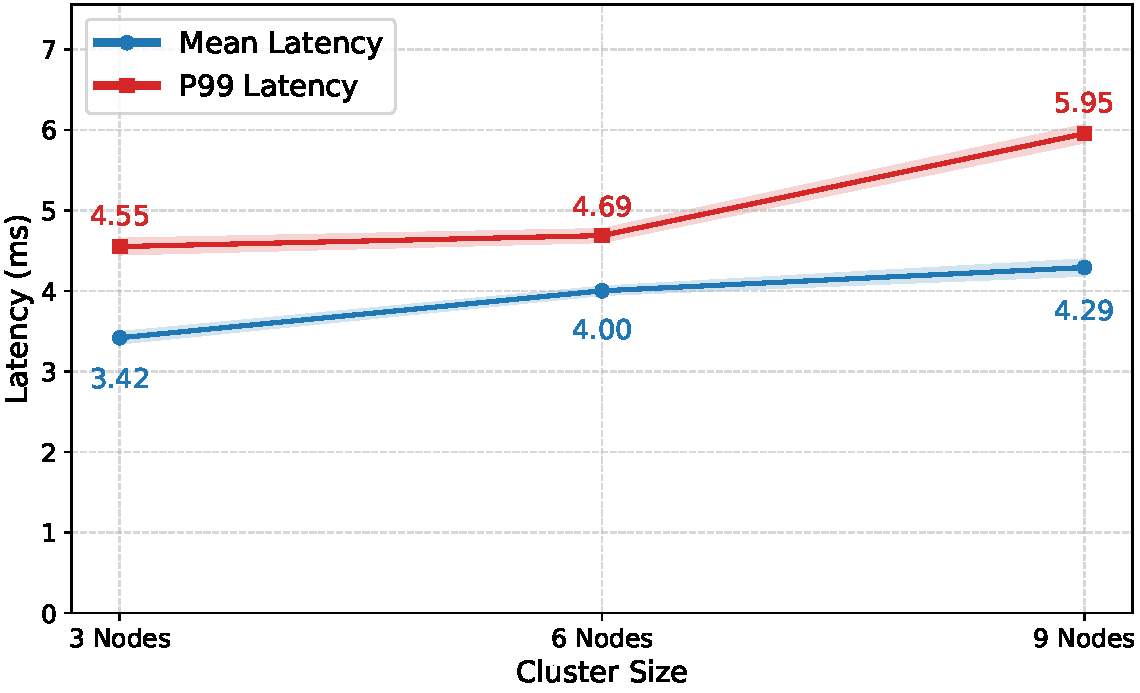
\includegraphics[width=\columnwidth]{../results/plots/3_consensus_tax.pdf}
\caption{Mean and P99 latency across cluster sizes. Shaded bands show inter-run standard deviation.}
\label{fig:consensus_tax}
\end{figure}

\subsection{Latency Under Load}
\label{subsec:latency_under_load}
The stress-latency experiment measures how latency degrades when the cluster is under heavy background load. A single publisher with synchronous confirms measures the latency while stress publishers flood the cluster using asynchronous confirms. Table~\ref{tab:stress_latency} summarizes the results.

\begin{table}[h]
\centering
\caption{Summary of results from the stress-latency experiment. Coverage shows the percentage of seconds in which at least one latency sample was recorded.}
\label{tab:stress_latency}
\begin{tabular}{l c c r}
\hline
\textbf{Cluster} & \textbf{Mean (ms)} & \textbf{P99 vs.\ Ideal P99} & \textbf{Coverage} \\
\hline
3 Nodes & 140.6 & 61$\times$  & 6.80\% (245/3607) \\
6 Nodes & 388.2 & 128$\times$ & 2.60\% (94/3608)  \\
9 Nodes & 611.9 & 146$\times$ & 1.64\% (59/3604)  \\
\hline
\end{tabular}
\end{table}

Latency under load is 61$\times$ to 146$\times$ worse than the ideal baseline (see Section~\ref{subsec:ideal_latency_results}). The low measurement coverage is not a measurement issue but a consequence of the experimental design. With synchronous confirms at 140--612\,ms per message, the measured publisher can only send approximately 2--7 messages per second. Since each CSV row aggregates a batch of 100 latency samples, filling one row takes 14--62 seconds, which matches the observed coverage ratios. The low inter-run standard deviation of the P99 values (5--27\,ms) shows that the system reaches a consistently degraded state across repeated runs rather than fluctuating unpredictably.

The large latency increase is likely caused by Erlang scheduler contention as CPU, disk and network all remain well below capacity (see Section~\ref{subsec:resource_utilization}). The stress publishers create heavy load across all nodes, including the node that hosts the measured queue's leader. Each quorum queue replica is limited to a single CPU core~\cite{rmq_queues_docs}, so the stress queue processes on the leader node compete with the measured queue's process for Erlang scheduler time. Although the stress publishers target separate queues, they slow down the measured queue's Raft process by consuming scheduler capacity on the same node. The RabbitMQ flow control mechanism further throttles publishers when internal buffers fill up~\cite{rmq_flow_control_docs}, adding to the latency increase.

Additionally, latency roughly quadruples from 3 to 9 nodes, growing faster than the cluster size itself. This is partly due to the quorum size increasing with the cluster size (from 3 to 9), which means more nodes must acknowledge each write under contention. However, the number of stress publishers also grows with the cluster size (10 per node, so 30 to 90 total), which means that the increased background load and the larger quorum both contribute to the latency degradation. Our experiment does not isolate these two factors, so the observed increase reflects the combined effect of more replication overhead and more resource contention. The stress-latency results demonstrate that when both quorum size and load grow with node count, latency degrades more than proportionally.

\begin{figure}[h]
\centering
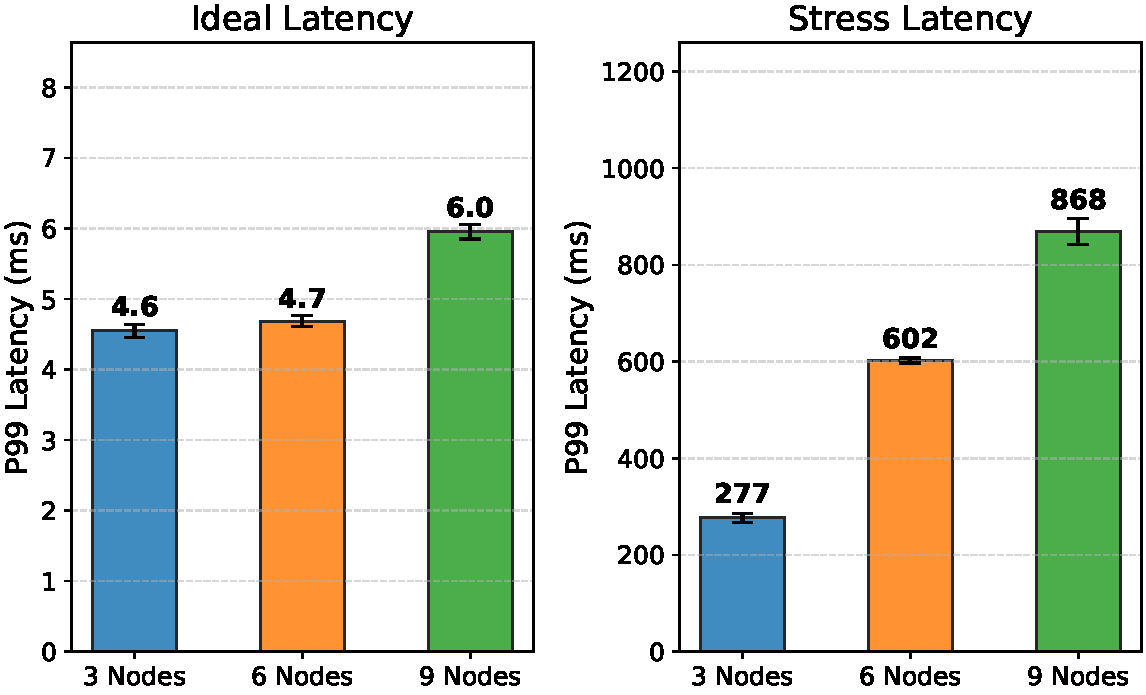
\includegraphics[width=\columnwidth]{../results/plots/2_latency_gradient.pdf}
\caption{Comparison of ideal (left) vs. stress (right) P99 latency. Note the different y-axis scales and error bars showing inter-run standard deviation.}
\label{fig:latency_gradient}
\end{figure}
\newpage

Figure~\ref{fig:latency_gradient} shows the contrast between ideal and stress P99 latency. The left panel shows ideal latency in the single-digit millisecond range while the right panel shows stress latency reaching hundreds of milliseconds.

\subsection{Resource Utilization}
\label{subsec:resource_utilization}
Figure~\ref{fig:resources} shows the cluster-wide average CPU utilization and total disk write throughput during the 9-node linear-capacity run, collected from Azure Monitor metrics. CPU averages around 60--65\% across the nine nodes throughout the benchmark. The total disk write throughput across all nodes is approximately 1{,}200\,MB/s, which corresponds to roughly 133\,MB/s per node and thus well below the 600\,MB/s provisioned per disk. Both metrics remain stable and demonstrate that the consistent throughput observed in Section~IV-A is matched by consistent resource consumption.

Network bandwidth is also not a limiting factor. Each D4s\_v6 node supports up to 12.5\,Gbps of network throughput and Azure Virtual Networks have no additional bandwidth limit. At the observed 9-node throughput of approximately 305{,}000 msgs/s with 1\,KB messages and a quorum size of 3, the total replication traffic is roughly 900\,MB/s across the cluster, or about 100\,MB/s per node, which is approximately 6\% of the per-node network capacity.

Neither CPU, disk I/O nor network are close to saturation, yet the per-node throughput peaks at approximately 34{,}000 msgs/s even after adding more publishers during the experiment. This suggests that the bottleneck lies within RabbitMQ's software architecture rather than the underlying hardware. As discussed in Section~\ref{subsec:latency_under_load}, each quorum queue replica is limited to a single CPU core. With four queues per node, only four leader processes handle the entire publishing load, which likely imposes the throughput ceiling before hardware resources are exhausted.

\begin{figure}[h]
\centering
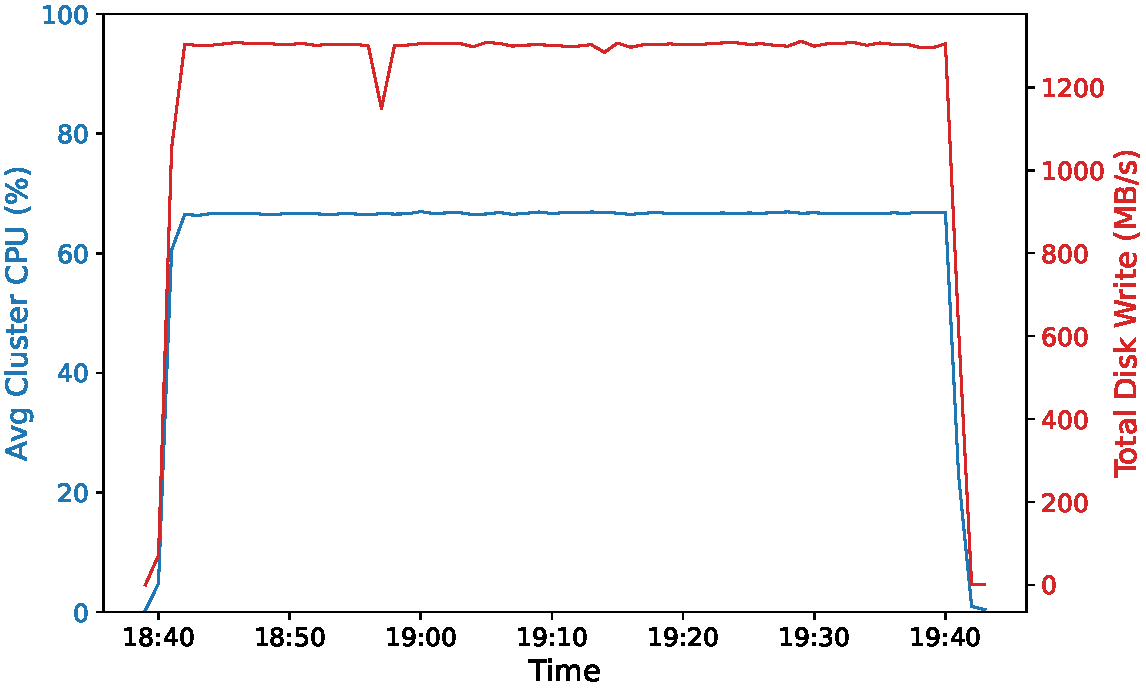
\includegraphics[width=\columnwidth]{../results/plots/4_resource_saturation.pdf}
\caption{Cluster-wide CPU utilization and disk write throughput during a single 9-node linear-capacity run.}
\label{fig:resources}
\end{figure}